\documentclass[11pt,a4paper]{article}

\usepackage[utf8]{inputenc}
\usepackage[T1]{fontenc}
\usepackage{lmodern}
\usepackage[margin=1in]{geometry}
\usepackage{hyperref}
\usepackage{booktabs}
\usepackage{longtable}
\usepackage{array}
\usepackage{tabularx}
\usepackage{enumitem}
\usepackage{xcolor}
\usepackage{listings}
\usepackage{amsmath}
\usepackage{amssymb}
\usepackage{graphicx}

\hypersetup{
  colorlinks=true,
  linkcolor=blue!50!black,
  urlcolor=blue!50!black
}

\lstset{
  basicstyle=\ttfamily\small,
  columns=fullflexible,
  keepspaces=true,
  breaklines=true,
  frame=single,
  framerule=0.3pt,
  showstringspaces=false
}

\setlist[itemize]{leftmargin=1.5em}
\setlist[enumerate]{leftmargin=1.8em}
\renewcommand{\arraystretch}{1.15}

\newcommand{\code}[1]{\texttt{\detokenize{#1}}}
\newcommand{\repo}{\texorpdfstring{\code{section_GNN}}{section_GNN}}

\title{Implementation-Level Documentation of \repo}
\author{Generated from the inspected repository state}
\date{March 31, 2026}

\begin{document}

\maketitle
\tableofcontents
\newpage

\section{Scope and Reading Contract}
This document describes the implementation that exists in the repository directory \code{section_GNN} as inspected on March 31, 2026. It is intentionally code-grounded rather than theoretical. Whenever the implementation and the surrounding documentation disagree, this report follows the Python source, YAML configuration, and generated artifacts currently present in the repository.

The codebase implements a leakage-aware legal outcome prediction pipeline built on PyTorch Geometric heterogeneous graphs. The main workflow is:

\begin{enumerate}
  \item load case JSON files produced by an upstream annotation pipeline,
  \item remove or mask decision-bearing text,
  \item normalize entities and derive a \code{CleanedCase} representation,
  \item build a per-case star graph,
  \item merge local graphs into a single heterogeneous graph,
  \item encode node text into dense vectors and append scalar features,
  \item train a hetero GNN to classify the \code{case} nodes,
  \item write metrics, predictions, plots, and visualization assets.
\end{enumerate}

Two shipped experiment families matter most in the current repository state:

\begin{itemize}
  \item \code{configs/gnn_case_star_food_law_final.yaml}: binary classification, labels \code{lose}/\code{win}, repeated training runs, sentence-transformer text embeddings.
  \item \code{configs/gnn_case_star_augmented_jsons_3way.yaml}: 3-way classification, labels \code{-1}/\code{0}/\code{1}, Hugging Face encoder backend, single training run.
\end{itemize}

\section{Repository Layout}

\subsection{Top-Level Structure}

\begin{lstlisting}
section_GNN/
  README.md
  configs/
    gnn_case_star.yaml
    gnn_case_star_food_law_final.yaml
    gnn_case_star_augmented_jsons_3way.yaml
    gnn_case_star_sanity.yaml
  envs/
    gnn_case_star.yaml
  scripts/
    preprocess_cases.py
    build_graph.py
    train_gnn.py
    run_ablation.py
    visualize_graph.py
    generate_final_visualisations.py
    export_visualiser_catalog.py
    export_training_graph_visualiser.py
  src/
    preprocessing/
    graph/
    models/
    training/
    utils/
    visualization/
  data/
    <experiment_name>/
      processed/
      audits/
      embeddings_cache/
      graph_cache/
  outputs/
    <experiment_name>/
      logs/
      models/
      ablations/
      visualizations/
  visualiser/
    index.html
    stats/index.html
    layers/index.html
    data/
  documentation/
    *.md
    section_gnn_documentation.tex
    section_gnn_documentation_slides.tex
\end{lstlisting}

\subsection{Directory Responsibilities}

\begin{tabularx}{\textwidth}{>{\raggedright\arraybackslash}p{0.18\textwidth}X}
\toprule
Directory or File Group & Responsibility \\
\midrule
\code{configs/} & Experiment configuration. Controls paths, preprocessing policy, graph topology, label mapping, split logic, model hyperparameters, and training schedule. \\
\code{envs/} & Micromamba/conda environment definition. Declares Python, PyTorch, PyG, scikit-learn, transformers, sentence-transformers, and plotting dependencies. \\
\code{scripts/} & User-facing entry points. These are the intended CLI commands for preprocessing, graph building, training, ablation, and visualization export. \\
\code{src/preprocessing/} & Input JSON loading, leakage phrase compilation and masking, annotation filtering, entity normalization, lawyer-side inference, role-specific argument extraction, and creation of \code{CleanedCase}. \\
\code{src/graph/} & Graph dataclasses, local case star construction, graph merging across cases, and conversion into PyG \code{HeteroData}. \\
\code{src/models/} & Neural model definitions: the hetero GNN backbone and the MLP classification head. \\
\code{src/training/} & Label preparation, split assignment, training loop, metric computation, and plotting utilities. \\
\code{src/utils/} & YAML/JSON I/O, deterministic seeding, logging, embedding cache logic, and pipeline orchestration. \\
\code{src/visualization/} & Static matplotlib/networkx explanatory figures that are separate from model training. \\
\code{visualiser/} & Browser-based D3 visualizer and supporting exported datasets. This is not part of model training, but it mirrors the graph structure for inspection. \\
\code{data/} & Experiment-local intermediate artifacts: cleaned JSON, audits, embedding caches, graph cache, and metadata. \\
\code{outputs/} & Experiment-local training products: logs, models, metrics, predictions, plots, repeated-run directories, ablation runs, and explanatory figures. \\
\bottomrule
\end{tabularx}

\subsection{Core Python Files}

\begin{longtable}{>{\raggedright\arraybackslash}p{0.28\textwidth}p{0.18\textwidth}p{0.45\textwidth}}
\toprule
File & Category & Implementation Role \\
\midrule
\endfirsthead
\toprule
File & Category & Implementation Role \\
\midrule
\endhead
\bottomrule
\endfoot
\code{src/preprocessing/loader.py} & preprocessing & Thin validation wrapper around JSON loading. Ensures each input file parses to a Python mapping. \\
\code{src/preprocessing/leakage.py} & preprocessing & Compiles leakage regexes, matches phrases, masks retained text, rejects suspicious annotations, and records leakage audit information. \\
\code{src/preprocessing/normalize.py} & preprocessing & Normalizes whitespace and entity names, removes honorifics for judges/lawyers, normalizes statute/provision forms, parses \code{provision &&& statute}, hashes petition type, and infers petition type from preamble text. \\
\code{src/preprocessing/extract.py} & preprocessing & Main preprocessing logic. Extracts leakage-safe text sections, derives \code{petitioner_arguments}/\code{respondent_arguments}/\code{other_lawyer_arguments}, maps annotation labels to graph node types, refines generic lawyers into side-specific lawyers, builds \code{CleanedCase.metadata}, and returns \code{CleanedCase}. \\
\code{src/graph/schema.py} & graph & Declares node-type constants, leakage defaults, dataclasses (\code{CleanedCase}, \code{EntityRecord}, \code{GraphNode}, \code{GraphEdge}, \code{CaseGraphSpec}), and a declarative relation catalog. \\
\code{src/graph/case_star_builder.py} & graph & Builds one local case graph from one \code{CleanedCase}. Creates text nodes, entity nodes, synthetic statute nodes, and all structural/citation/bridging edges. \\
\code{src/graph/global_graph_builder.py} & graph & Deduplicates shareable nodes and edges across case graphs, aggregates metadata such as \code{global_case_frequency} and node degree, and produces the global graph registries. \\
\code{src/graph/pyg_builder.py} & graph & Encodes every node into a numeric feature vector, creates PyG \code{HeteroData}, attaches labels and split masks to case nodes, optionally makes the graph undirected, and emits graph metadata. \\
\code{src/models/mlp_head.py} & model & Two-layer classifier head: \code{Linear -> ReLU -> Dropout -> Linear}. \\
\code{src/models/hetero_gnn.py} & model & \code{HeteroLegalOutcomeGNN}. Performs node-type-specific input projection, adds learned type embeddings, applies either \code{HGTConv} or \code{HeteroConv(SAGEConv)} stacks, normalizes with residuals, and classifies the case nodes. \\
\code{src/training/dataset.py} & training & Maps raw labels to class indices, optionally drops procedural cases, and builds train/val/test assignments using either random or grouped splits. \\
\code{src/training/train.py} & training & Full-graph training loop, class-weight computation, validation model selection, early stopping, final evaluation, and prediction table generation. \\
\code{src/training/evaluate.py} & training & Very small wrapper that handles empty splits and delegates to \code{compute_metrics}. \\
\code{src/training/metrics.py} & training & Computes accuracy/F1/confusion/class reports and writes confusion matrices, training-history plots, and split metric bar charts. \\
\code{src/utils/io.py} & utils & JSON/YAML read/write, directory creation, file listing, and recursive config merge for ablations. \\
\code{src/utils/seed.py} & utils & Global deterministic seeding for Python, NumPy, and PyTorch. Enables deterministic CUDA algorithms when available. \\
\code{src/utils/logging_utils.py} & utils & Configures stdout and file logging with a uniform timestamped format. \\
\code{src/utils/text_encoder.py} & utils & Text encoder backends (\code{SentenceTransformerEncoder}, \code{HFEncoder}, \code{HashingEncoder}), embedding caching, and backend fallback. \\
\code{src/utils/pipeline.py} & utils & Orchestrates cleaned-case loading, integrity assertions, graph bundle creation, split assignment, and debug metadata assembly. \\
\code{src/visualization/graph_visualizer.py} & visualization & Generates explanatory static figures for graph schema, local case stars, receptive field views, and message-passing diagrams. \\
\code{src/visualization/final_visualizer.py} & visualization & Generates explanatory figures about what is stored in nodes and edges, how layers update the case node, and how training uses labels. \\
\code{scripts/preprocess_cases.py} & script & CLI entry point for producing cleaned cases, normalized entities, audits, and \code{preprocess_summary.json}. \\
\code{scripts/build_graph.py} & script & CLI entry point for producing a serialized graph bundle and metadata snapshots. \\
\code{scripts/train_gnn.py} & script & CLI entry point for training once or for repeated runs, selecting the best run, and writing model outputs. \\
\code{scripts/run_ablation.py} & script & Builds and trains multiple graph variants by merging base config with ablation overrides. \\
\code{scripts/visualize_graph.py} & script & Generates static schema/case/receptive-field figures plus a simplified visual guide. \\
\code{scripts/generate_final_visualisations.py} & script & Generates final presentation-style explanatory images focused on vertex storage, edge storage, layer 1, layer 2, and label use. \\
\code{scripts/export_visualiser_catalog.py} & script & Exports a sampled browser-friendly case catalog for the static D3 visualizer. \\
\code{scripts/export_training_graph_visualiser.py} & script & Exports exact per-case training-graph JSON files so the browser visualizer can show the real local graph used in training. \\
\end{longtable}

\section{End-to-End Pipeline}

\subsection{Stage-by-Stage Execution}

\begin{enumerate}
  \item \textbf{Raw JSON loading.} \code{scripts/preprocess_cases.py} scans \code{paths.raw_json_dir}, loads each JSON with \code{load_case_json()}, and passes it to \code{clean_case_for_gnn()}.
  \item \textbf{Leakage-safe text extraction.} \code{extract_prejudgment_text()} reads \code{raw_result.summary}, optionally falls back to annotation text, removes or masks leakage phrases, and derives the six retained text fields:
  \begin{itemize}
    \item \code{preamble}
    \item \code{facts}
    \item \code{arguments}
    \item \code{petitioner_arguments}
    \item \code{respondent_arguments}
    \item \code{other_lawyer_arguments}
  \end{itemize}
  \item \textbf{Entity extraction and normalization.} \code{extract_entities_from_annotations()} filters annotations by section, forbidden labels, and leakage matches; maps upstream labels to internal node types; normalizes entity names; refines generic lawyers to side-specific lawyers; and builds \code{EntityRecord} objects.
  \item \textbf{Per-case serialization.} The preprocessing script writes:
  \begin{itemize}
    \item cleaned cases to \code{processed/cleaned_cases/*.json},
    \item normalized entities to \code{processed/normalized_entities/*.json},
    \item leakage audits to \code{audits/*.json},
    \item a dataset-level summary to \code{processed/preprocess_summary.json}.
  \end{itemize}
  \item \textbf{Task filtering and label mapping.} \code{prepare_cases_for_task()} turns raw labels into class indices and drops unmapped cases when the active task says to do so.
  \item \textbf{Local graph construction.} \code{build_case_star_graph()} builds one \code{CaseGraphSpec} per retained case.
  \item \textbf{Global graph construction.} \code{merge_case_graphs_into_global_graph()} merges shareable nodes across cases and computes global frequencies and degrees.
  \item \textbf{PyG conversion.} \code{build_pyg_heterodata()} embeds node text, appends scalar features, attaches labels and split masks to case nodes, and emits a \code{HeteroData} object plus graph metadata.
  \item \textbf{Training.} \code{train_model()} loads the entire graph on one device, computes logits for all case nodes, applies loss only on \code{train_mask}, selects the best epoch by validation macro F1, and then evaluates train/val/test on the best checkpoint.
  \item \textbf{Artifact writing.} \code{scripts/train_gnn.py} writes \code{model.pt}, \code{metrics.json}, \code{predictions.csv}, \code{history.csv}, confusion matrices, training-history plots, and repeated-run summaries when enabled.
\end{enumerate}

\subsection{The Three Main Entry Points}

\begin{enumerate}
  \item \code{python scripts/preprocess_cases.py --config <config.yaml>}
  \item \code{python scripts/build_graph.py --config <config.yaml>}
  \item \code{python scripts/train_gnn.py --config <config.yaml> --run-name <name>}
\end{enumerate}

The codebase is designed so these three scripts are the normal reproducible pipeline boundary. Everything else is either ablation, visualization, or browser-export support.

\subsection{Generated Cross-Repository Pipeline Figure}
The file \code{scripts/generate_documentation_diagrams.py} generates a cross-repository figure that starts in \code{Fixed_GPU_OpenNyai} and ends in \repo{}. It is intended to make the handoff explicit: OpenNyAI produces wrapped combined JSONs, the Mistral labeller adds outcome supervision, and \repo{} then strips the leakage-bearing fields back out before graph construction.

\begin{figure}[p]
  \centering
  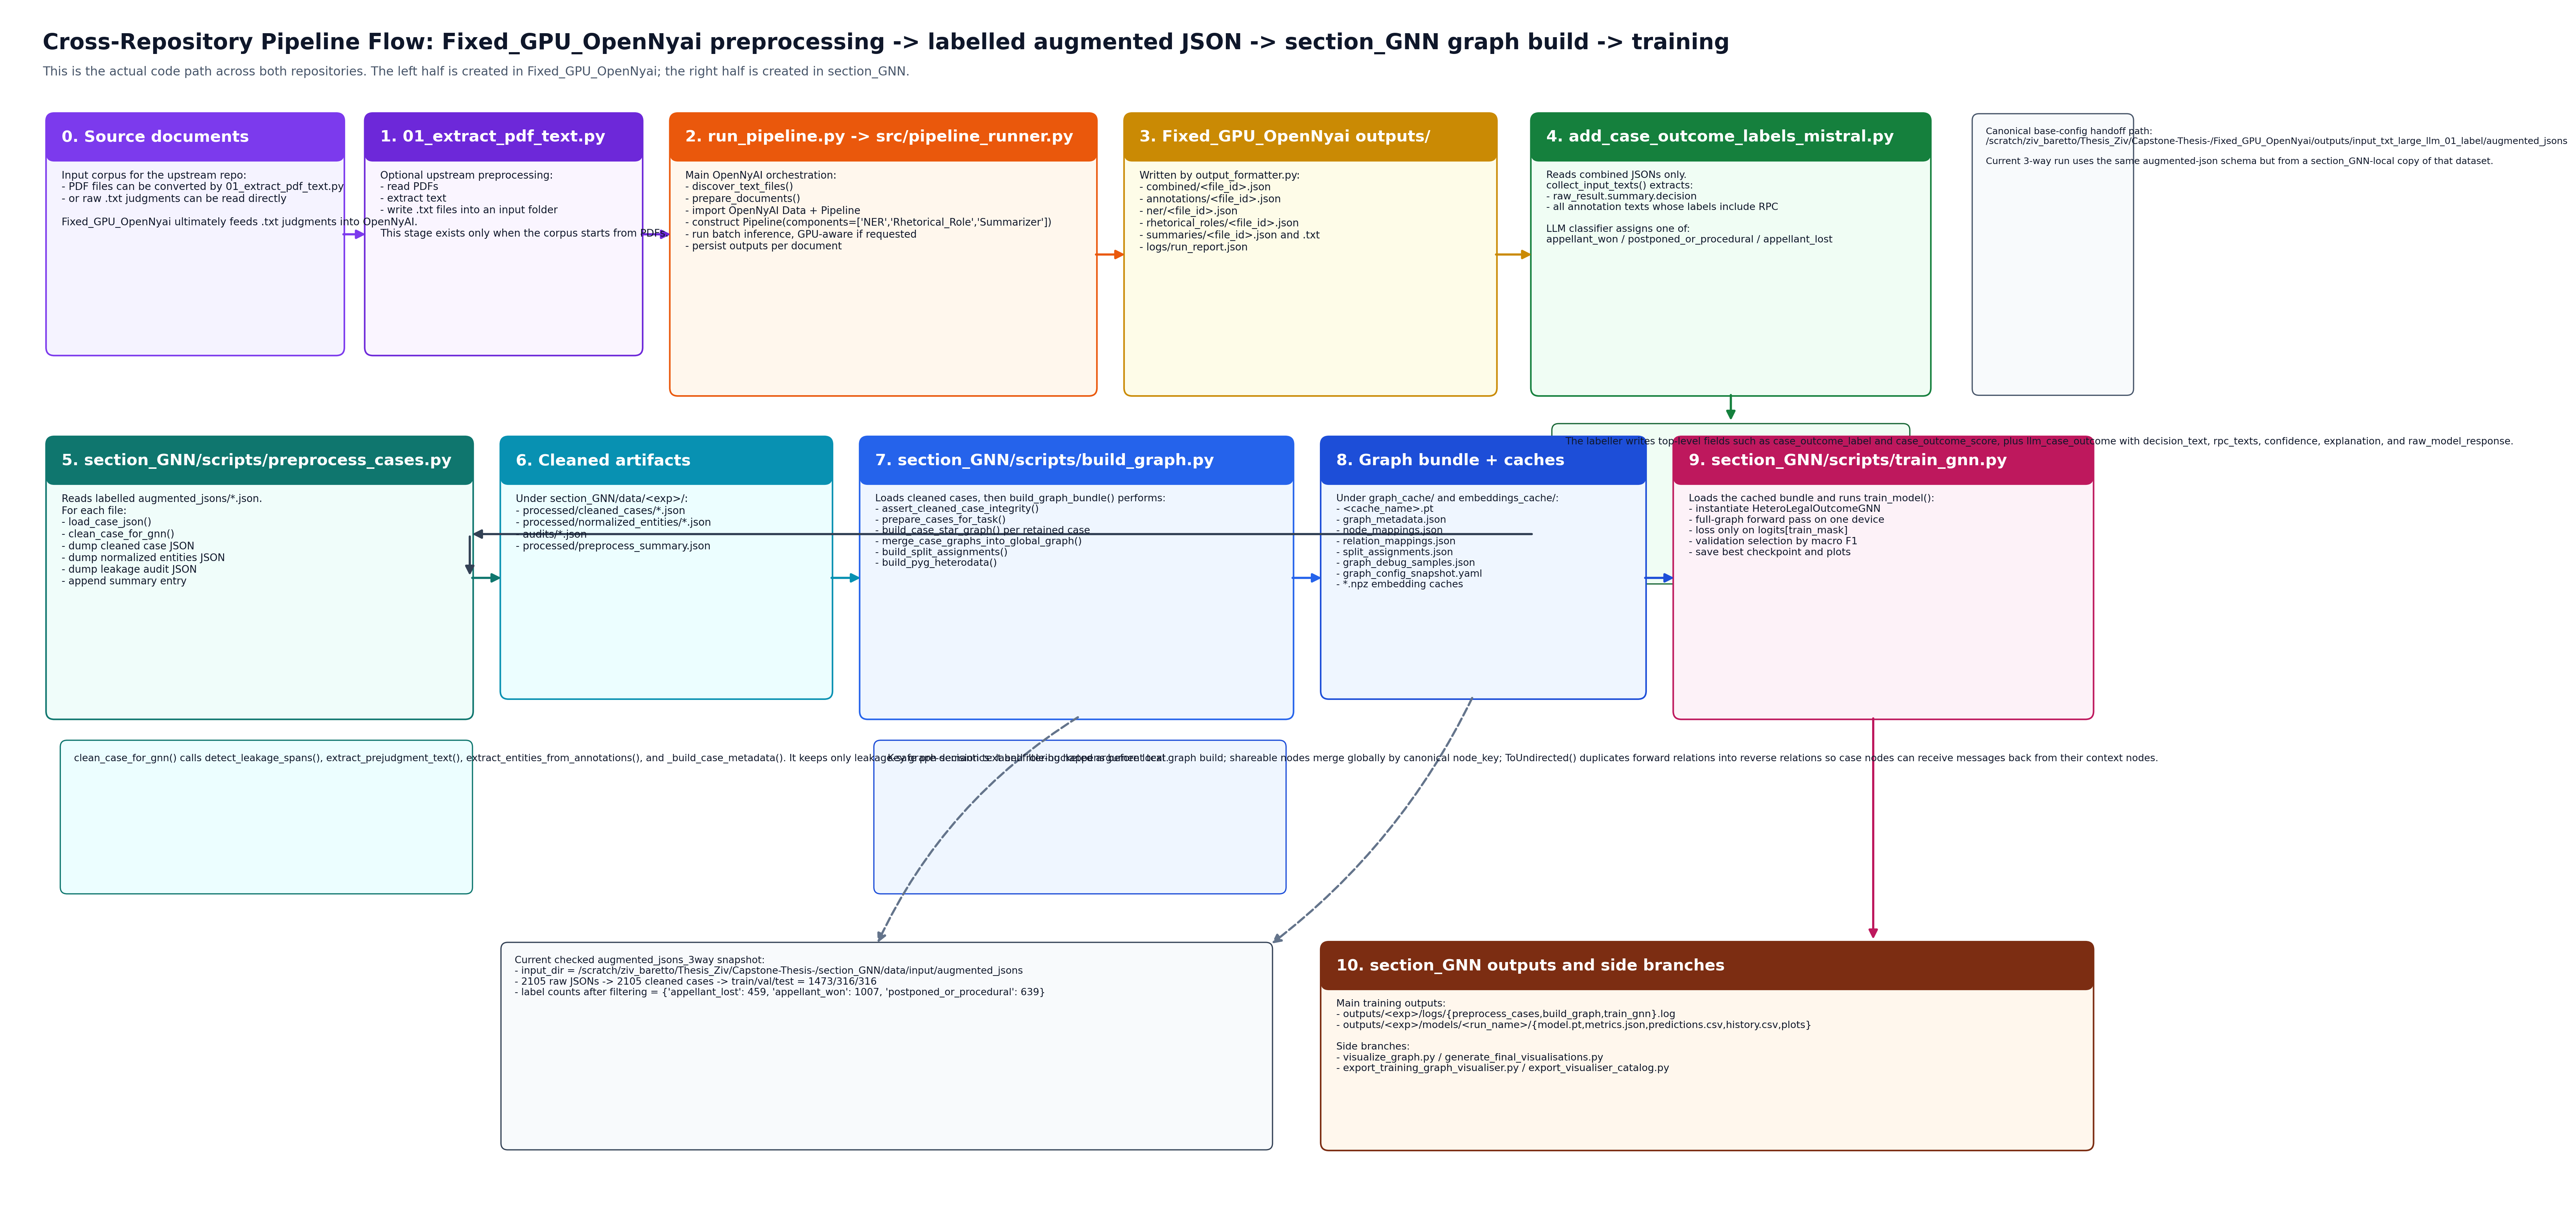
\includegraphics[width=\textwidth]{figures/section_gnn_pipeline_flow.png}
  \caption{Exact cross-repository data flow from \code{Fixed_GPU_OpenNyai} into \repo{}, including the OpenNyAI output formatter, LLM outcome labeller, leakage-safe preprocessing, graph caching, and model training.}
  \label{fig:section-gnn-pipeline-flow}
\end{figure}

\section{Data Formats and Schemas}

\subsection{Expected Raw Input JSON Contract}
The pipeline is tolerant of missing keys because it uses \code{dict.get()} extensively, but the implemented logic expects the following structure:

\begin{lstlisting}
{
  "file_id": "...",
  "internal_file_id": "...",
  "source_path": "...",
  "case_outcome_label": "appellant_won | appellant_lost | postponed_or_procedural",
  "raw_result": {
    "summary": {
      "PREAMBLE": "...",
      "facts": "...",
      "arguments": "...",
      "decision": "..."
    },
    "data": {
      "text": "...",
      "preamble_end_char_offset": 1234
    },
    "annotations": [
      {
        "id": "...",
        "summary_section": "PREAMBLE | facts | arguments | decision | ...",
        "labels": ["..."],
        "text": "...",
        "entities": [
          {
            "text": "...",
            "normalized_name": "...",
            "labels": ["LAWYER", "..."],
            "start": 10,
            "end": 25
          }
        ]
      }
    ]
  }
}
\end{lstlisting}

\subsection{What the Preprocessing Layer Keeps and Drops}

\begin{tabularx}{\textwidth}{>{\raggedright\arraybackslash}p{0.28\textwidth}X}
\toprule
Item & Implemented Behavior \\
\midrule
Top-level fields such as \code{case_outcome_label}, \code{case_outcome_score}, \code{llm_case_outcome}, \code{decision_text}, \code{rpc_texts}, \code{short_explanation}, \code{raw_model_response} & Recorded as dropped in the leakage audit and not copied into \code{CleanedCase.texts}. \\
\code{raw_result.summary.decision} & Treated as removed decision text and recorded in the audit. \\
Annotations in sections \code{decision}, \code{ANALYSIS}, or \code{issue} & Rejected by \code{is_forbidden_annotation()}. \\
Annotations with labels \code{RPC} or \code{RLC} & Rejected by \code{is_forbidden_annotation()}. \\
Annotations whose text matches any configured leakage phrase & Rejected. \\
Retained preamble/facts/arguments text that still contains leakage phrases & Phrase occurrences are replaced with \code{[LEAKAGE_MASK]}. \\
\bottomrule
\end{tabularx}

\subsection{Leakage Phrase Policy}
Leakage phrases are compiled by \code{compile_leakage_patterns()} into case-insensitive word-boundary regexes. The default phrase list includes strings such as:

\begin{itemize}
  \item \code{appeal is allowed}
  \item \code{appeal dismissed}
  \item \code{petition dismissed}
  \item \code{set aside}
  \item \code{quashed}
  \item \code{liberty granted}
\end{itemize}

This policy is literal and phrase-driven. There is no learned leakage detector and no semantic paraphrase detector.

\subsection{The \code{CleanedCase} Schema}
\code{CleanedCase} is the canonical intermediate representation used by graph construction.

\begin{longtable}{>{\raggedright\arraybackslash}p{0.24\textwidth}p{0.20\textwidth}p{0.46\textwidth}}
\toprule
Field & Type & Meaning \\
\midrule
\endfirsthead
\toprule
Field & Type & Meaning \\
\midrule
\endhead
\bottomrule
\endfoot
\code{case_id} & string & Derived from the input file stem. Used everywhere as the stable case identifier. \\
\code{file_name} & string & Original JSON filename. \\
\code{file_id} & string or null & Passed through from the source JSON when present. \\
\code{internal_file_id} & string or null & Passed through from the source JSON when present. \\
\code{source_path} & string or null & Original source path, if provided by upstream data. \\
\code{raw_label} & string or null & The original case outcome label from the raw JSON. This is the supervision source before mapping. \\
\code{texts} & mapping & Leakage-safe retained text sections. Keys may include \code{preamble}, \code{facts}, \code{arguments}, \code{petitioner_arguments}, \code{respondent_arguments}, \code{other_lawyer_arguments}. \\
\code{metadata} & mapping & Numeric and categorical per-case metadata built by \code{_build_case_metadata()}. Includes counts, lengths, inferred year, petition type, and short normalized name lists for courts/judges/statutes. \\
\code{entities} & list of \code{EntityRecord} & Normalized entities extracted from retained annotations. \\
\code{leakage_audit} & mapping & Audit payload combining dropped fields, dropped annotations, retained-text source and length info, and entity extraction audit. \\
\end{longtable}

\subsection{The \code{EntityRecord} and \code{EntityMention} Schemas}

\begin{itemize}
  \item \code{EntityMention} stores \code{entity_type}, \code{raw_text}, \code{canonical_text}, \code{section}, \code{annotation_id}, \code{start}, and \code{end}.
  \item \code{EntityRecord} stores the normalized entity aggregate for one case:
  \begin{itemize}
    \item \code{entity_type}
    \item \code{raw_name}
    \item \code{canonical_name}
    \item \code{mentions}
    \item \code{local_case_frequency}
    \item \code{first_seen_section}
    \item \code{seen_in_arguments}
    \item \code{seen_in_preamble}
    \item \code{linked_statute_canonical} for provision nodes when the source annotation encoded a \code{provision &&& statute} pair
  \end{itemize}
\end{itemize}

\subsection{Per-Case Metadata Built in \code{extract.py}}
For every cleaned case, the preprocessing layer computes:

\begin{itemize}
  \item entity counts: respondents, judges, lawyers, statutes, provisions, precedents, courts,
  \item section lengths: preamble, facts, arguments,
  \item \code{case_year}: the first year parsed from a \code{date} entity containing at least four digits,
  \item \code{petition_type}: inferred from preamble text using markers such as \code{writ petition}, \code{appeal}, \code{bail application}, etc.,
  \item \code{petition_type_hash}: stable hash in the unit interval,
  \item short normalized name lists: \code{court_names}, \code{judge_names}, \code{statute_names}.
\end{itemize}

\subsection{Other On-Disk Schemas Produced by the Pipeline}

\begin{tabularx}{\textwidth}{>{\raggedright\arraybackslash}p{0.30\textwidth}X}
\toprule
Artifact & Contents \\
\midrule
\code{processed/preprocess_summary.json} & Dataset-level summary with one row per processed file: case id, raw label, retained text lengths, dropped top-level fields, and dropped annotation count. \\
\code{processed/normalized_entities/*.json} & Simplified file containing \code{case_id} and the list of normalized entities. \\
\code{audits/*.json} & Per-case leakage audit, including dropped annotations, matched leakage phrases, and text-source tracing. \\
\code{graph_cache/*.pt} & A \code{torch.save()} bundle with two keys: \code{data} (\code{HeteroData}) and \code{metadata} (Python dict). \\
\code{graph_cache/graph_metadata.json} & Serialized graph metadata, including label names, feature dimension, relation names, split counts, node counts, dropped case ids, and relation statistics. \\
\code{graph_cache/node_mappings.json} & Mapping from each node type and node key to its integer row index inside PyG. \\
\code{graph_cache/relation_mappings.json} & Stringified edge types exactly as present in \code{data.edge_types}. \\
\code{graph_cache/split_assignments.json} & Case-id to split-name mapping. Only retained cases are present. \\
\code{graph_cache/graph_debug_samples.json} & Lightweight debug view of the first configured sample cases after label filtering. \\
\bottomrule
\end{tabularx}

\section{Preprocessing Implementation Details}

\subsection{Allowed Entity Labels}
\code{extract.py} maps the following upstream labels to internal node types:

\begin{center}
\begin{tabular}{ll}
\toprule
Upstream label & Internal node type \\
\midrule
\code{PETITIONER} & \code{petitioner} \\
\code{RESPONDENT} & \code{respondent} \\
\code{COURT} & \code{court} \\
\code{JUDGE} & \code{judge} \\
\code{LAWYER} & initially \code{lawyer}, then refined by context \\
\code{STATUTE} & \code{statute} \\
\code{PROVISION} & \code{provision} \\
\code{CASE_NUMBER} & \code{case_number} \\
\code{DATE} & \code{date} \\
\code{ORG} & \code{org} \\
\code{GPE} & \code{gpe} \\
\code{PRECEDENT} & \code{precedent} \\
\bottomrule
\end{tabular}
\end{center}

Any other annotation label is ignored and recorded in the entity-extraction audit.

\subsection{Lawyer-Side Inference}
The code does not rely on a dedicated upstream petitioner-lawyer or respondent-lawyer label. Instead:

\begin{enumerate}
  \item \code{LAWYER} annotations are first mapped to the generic internal type \code{lawyer}.
  \item \code{_infer_lawyer_side()} inspects a local character window around the mention:
  \begin{itemize}
    \item up to 300 characters before the mention,
    \item up to 150 characters after the mention.
  \end{itemize}
  \item If petitioner/appellant phrases are found, the entity is retyped to \code{petitioner_lawyer}.
  \item If respondent/state phrases are found, the entity is retyped to \code{defence_lawyer}.
  \item Otherwise it remains \code{lawyer}.
\end{enumerate}

Examples of petitioner signals include \code{for petitioner}, \code{for appellant}, \code{counsel for petitioner}. Examples of respondent signals include \code{for respondent}, \code{public prosecutor}, \code{government pleader}, \code{a.g.a.}, and \code{a.p.p.}.

\subsection{Role-Specific Argument Bucketing}
When \code{derive_role_argument_sections} is enabled, \code{extract.py} also derives three optional argument sub-sections from annotations whose \code{summary_section} is \code{arguments}:

\begin{itemize}
  \item \code{petitioner_arguments}
  \item \code{respondent_arguments}
  \item \code{other_lawyer_arguments}
\end{itemize}

Bucketing is done in two ways:

\begin{enumerate}
  \item by scanning lawyer entities already present in the annotation and reusing the side-inference logic;
  \item by scanning the annotation text itself for petitioner, respondent, or generic-counsel signal phrases.
\end{enumerate}

If no bucket can be inferred, the annotation stays only in the general \code{arguments} text and is not copied into a role-specific section.

\subsection{Normalization Rules}

\begin{itemize}
  \item whitespace is collapsed everywhere;
  \item judges and lawyers have honorifics such as \code{Justice}, \code{Mr}, \code{Mrs}, \code{Dr}, \code{Advocate}, \code{Sr.}, \code{Jr.} stripped before punctuation removal;
  \item court names have some repeated boilerplate reduced, such as replacing \code{high court of judicature at} with \code{high court at};
  \item statutes and provisions normalize abbreviations like \code{sec.}, \code{u/s}, and \code{cr.p.c.};
  \item punctuation is removed for most entity types except \code{case_number}, \code{date}, and \code{provision}.
\end{itemize}

\subsection{One Concrete Cleaned-Case Example}
In the current 3-way processed dataset, the file
\code{data/augmented_jsons_3way/processed/cleaned_cases/A_Biswanath_Patra_vs_State_Of_Odisha_Ors_Opposite_on_5_February_2024.json}
contains:

\begin{itemize}
  \item raw label \code{appellant_lost},
  \item all six retained text fields, including non-empty \code{petitioner_arguments} and \code{respondent_arguments},
  \item metadata values such as \code{judge_count = 3}, \code{statute_count = 1}, \code{provision_count = 2}, \code{case_year = 2024},
  \item 18 extracted normalized entities.
\end{itemize}

\section{Graph Construction}

\subsection{Build Modes}
\code{build_case_star_graph()} accepts three operational modes via \code{graph.build_mode}:

\begin{center}
\begin{tabular}{lp{0.66\textwidth}}
\toprule
Mode & Implemented Behavior \\
\midrule
\code{full_star_global} & Full graph. Text nodes and entity nodes are created. Shareable node types may merge across cases. This is the normal mode. \\
\code{text_only} & Only the case node and configured text nodes are created. The entire entity loop is skipped. \\
\code{local_star_only} & Text nodes and entity nodes are created, but shareability is forcibly disabled even for normally shareable types. \\
\bottomrule
\end{tabular}
\end{center}

\subsection{Node-Key Strategy}
Node identity is determined by \code{_node_key()}:

\begin{itemize}
  \item shared nodes use \code{<node_type>::<canonical_name>},
  \item case-local nodes use \code{case::<case_id>::<node_type>::<canonical_name>},
  \item the case node itself always uses \code{case::<case_id>},
  \item text nodes use \code{case::<case_id>::<section_name>}.
\end{itemize}

This is the mechanism that turns selected entity types into cross-case bridges.

\subsection{Every Node Type and Its Meaning}

\begin{longtable}{>{\raggedright\arraybackslash}p{0.18\textwidth}p{0.19\textwidth}p{0.21\textwidth}p{0.33\textwidth}}
\toprule
Node type & Source & Shared by default? & Meaning in this codebase \\
\midrule
\endfirsthead
\toprule
Node type & Source & Shared by default? & Meaning in this codebase \\
\midrule
\endhead
\bottomrule
\endfoot
\code{case} & one per retained case & no & Root prediction target. Its text is the concatenation of configured base text sections (\code{preamble}, \code{facts}, \code{arguments}) and its metadata carries case-level counts, lengths, year, petition type, file name, and raw label. \\
\code{preamble} & retained text section & no & Case header and opening material. Created only if included by config and non-empty. \\
\code{facts} & retained text section & no & Facts summary retained after leakage masking. Created only if included and non-empty. \\
\code{arguments} & retained text section & no & General arguments summary retained after leakage masking. This is the hub for citations and several bridging edges. \\
\code{petitioner_arguments} & derived text section & no & Argument text inferred to belong to the petitioner/appellant side. \\
\code{respondent_arguments} & derived text section & no & Argument text inferred to belong to the respondent/state side. \\
\code{other_lawyer_arguments} & derived text section & no & Argument text associated with lawyers but not confidently assigned to petitioner or respondent. \\
\code{petitioner} & annotation entities & no by default & Named petitioner entity. Can be made shareable only when \code{share_party_nodes: true}. \\
\code{respondent} & annotation entities & no by default & Named respondent entity. Can be made shareable only when \code{share_party_nodes: true}. \\
\code{court} & annotation entities & yes in shipped graph configs & Normalized court or bench. Major cross-case authority node. \\
\code{judge} & annotation entities & yes in shipped graph configs & Normalized judge name. Cross-case bridge. \\
\code{petitioner_lawyer} & annotation entities after side refinement & yes in shipped graph configs & Lawyer mention inferred to represent the petitioner/appellant side. \\
\code{defence_lawyer} & annotation entities after side refinement & yes in shipped graph configs & Lawyer mention inferred to represent the respondent/state side. The spelling in code is \code{defence_lawyer}. \\
\code{lawyer} & annotation entities after side refinement & yes in shipped graph configs & Lawyer mention not confidently assigned to either side. \\
\code{statute} & annotation entities or synthetic node from provision linkage & yes in shipped graph configs & Normalized legislation reference. May be synthetic when only a provision mention carried the statute name. \\
\code{provision} & annotation entities & yes in shipped graph configs & Normalized section/rule/provision citation. Can also link upward to a statute via \code{belongs_to_statute}. \\
\code{precedent} & annotation entities & yes in shipped graph configs & Prior-case citation appearing in arguments. \\
\code{org} & annotation entities & yes in shipped graph configs & Organization mention. \\
\code{gpe} & annotation entities & yes in shipped graph configs & Geopolitical/place entity. \\
\code{date} & annotation entities & yes in shipped graph configs & Date mention. Used both as graph context and for heuristic year extraction. \\
\code{case_number} & annotation entities & yes in shipped graph configs & Case/FIR/reference number mention. \\
\end{longtable}

\subsection{Node Metadata}
\paragraph{Case node metadata.}
The case node stores:

\begin{itemize}
  \item all values from \code{cleaned_case.metadata},
  \item \code{case_id},
  \item \code{file_name},
  \item \code{raw_label},
  \item \code{text_sections}, a mapping of included section names to retained text.
\end{itemize}

\paragraph{Text node metadata.}
Each text node stores:

\begin{itemize}
  \item \code{case_id},
  \item \code{section},
  \item \code{text_length},
  \item counters initialized to zero and later interpreted as argument citation/bridge counts:
  \begin{itemize}
    \item \code{cited_statute_count}
    \item \code{cited_provision_count}
    \item \code{cited_precedent_count}
    \item \code{petitioner_lawyer_count}
    \item \code{defence_lawyer_count}
    \item \code{petitioner_count}
    \item \code{respondent_count}
    \item \code{judge_count}
  \end{itemize}
\end{itemize}

\paragraph{Entity node metadata.}
Each entity node stores:

\begin{itemize}
  \item \code{case_id},
  \item \code{raw_name},
  \item \code{canonical_name},
  \item \code{mention_count},
  \item \code{first_seen_section},
  \item \code{seen_in_arguments},
  \item \code{seen_in_preamble},
  \item \code{linked_statute_canonical},
  \item \code{is_shared_node}.
\end{itemize}

Synthetic statute nodes created from provision metadata additionally set \code{synthetic_from_provision: true}.

\subsection{Every Forward Edge Type and Its Meaning}
The runtime graph builder creates the following forward edge types. Reverse edges are not created here; they are added later by \code{ToUndirected}.

\begin{longtable}{>{\raggedright\arraybackslash}p{0.16\textwidth}p{0.25\textwidth}p{0.16\textwidth}p{0.34\textwidth}}
\toprule
Source & Relation & Target & Meaning and creation rule \\
\midrule
\endfirsthead
\toprule
Source & Relation & Target & Meaning and creation rule \\
\midrule
\endhead
\bottomrule
\endfoot
\code{case} & \code{has_preamble} & \code{preamble} & Connects the case root to the retained preamble section. \\
\code{case} & \code{has_facts} & \code{facts} & Connects the case root to the retained facts section. \\
\code{case} & \code{has_arguments} & \code{arguments} & Connects the case root to the retained generic arguments section. \\
\code{case} & \code{has_petitioner_arguments} & \code{petitioner_arguments} & Connects the case root to the petitioner-side argument bucket. \\
\code{case} & \code{has_respondent_arguments} & \code{respondent_arguments} & Connects the case root to the respondent-side argument bucket. \\
\code{case} & \code{has_other_lawyer_arguments} & \code{other_lawyer_arguments} & Connects the case root to the unassigned-lawyer argument bucket. \\
\code{case} & \code{has_petitioner} & \code{petitioner} & Connects the case to petitioner entities. \\
\code{case} & \code{has_respondent} & \code{respondent} & Connects the case to respondent entities. \\
\code{case} & \code{heard_in} & \code{court} & Connects the case to the court/bench. \\
\code{case} & \code{decided_by_bench} & \code{judge} & Connects the case to judges. \\
\code{case} & \code{has_lawyer} & \code{lawyer} & Connects the case to generic lawyers. \\
\code{case} & \code{has_petitioner_lawyer} & \code{petitioner_lawyer} & Connects the case to petitioner-side lawyers. \\
\code{case} & \code{has_defence_lawyer} & \code{defence_lawyer} & Connects the case to respondent-side lawyers. \\
\code{case} & \code{mentions_org} & \code{org} & Connects the case to organization mentions. \\
\code{case} & \code{mentions_gpe} & \code{gpe} & Connects the case to place/geopolitical mentions. \\
\code{case} & \code{has_case_number} & \code{case_number} & Connects the case to case-number/reference entities. \\
\code{case} & \code{has_date} & \code{date} & Connects the case to date mentions. \\
\code{arguments} & \code{cites_statute} & \code{statute} & Added when a statute entity was seen in arguments and the generic arguments node exists. \\
\code{arguments} & \code{cites_provision} & \code{provision} & Added when a provision entity was seen in arguments and the generic arguments node exists. \\
\code{arguments} & \code{cites_precedent} & \code{precedent} & Added when a precedent entity was seen in arguments and the generic arguments node exists. \\
\code{provision} & \code{belongs_to_statute} & \code{statute} & Added when a provision carried a linked statute canonical name, even if the statute node had to be created synthetically. \\
\code{petitioner_lawyer} & \code{citation} & \code{arguments} & Generic bridge from petitioner-side lawyer to the general arguments node when the lawyer was seen in arguments. \\
\code{defence_lawyer} & \code{citation} & \code{arguments} & Generic bridge from respondent-side lawyer to the general arguments node when the lawyer was seen in arguments. \\
\code{petitioner_lawyer} & \code{citation} & \code{petitioner_arguments} & Side-specific bridge into the petitioner arguments bucket when that bucket exists. \\
\code{defence_lawyer} & \code{citation} & \code{respondent_arguments} & Side-specific bridge into the respondent arguments bucket when that bucket exists. \\
\code{lawyer} & \code{citation} & \code{other_lawyer_arguments} & Bridge from generic lawyer to unassigned-lawyer argument text when that bucket exists. \\
\code{provision} & \code{used_in_arguments} & \code{arguments} & Shortens the path from a provision to the generic arguments node. \\
\code{statute} & \code{used_in_arguments} & \code{arguments} & Shortens the path from a statute to the generic arguments node. \\
\code{petitioner} & \code{is_party_in_arguments} & \code{arguments} & Bridges petitioner entity into the generic arguments node. \\
\code{respondent} & \code{is_party_in_arguments} & \code{arguments} & Bridges respondent entity into the generic arguments node. \\
\code{petitioner} & \code{is_party_in_arguments} & \code{petitioner_arguments} & Bridges petitioner entity into the petitioner-specific arguments node. \\
\code{respondent} & \code{is_party_in_arguments} & \code{respondent_arguments} & Bridges respondent entity into the respondent-specific arguments node. \\
\code{judge} & \code{presided_arguments} & \code{arguments} & Bridges judge entity into the generic arguments node. \\
\end{longtable}

\subsection{Reverse Edges}
If \code{graph.use_to_undirected} is true, \code{build_pyg_heterodata()} applies \code{torch_geometric.transforms.ToUndirected}. This duplicates every forward relation with a reverse relation named \code{rev_<relation>}. In the current shipped binary and 3-way graph caches, this produces:

\begin{itemize}
  \item 33 forward relation types,
  \item 33 reverse relation types,
  \item 66 total relation types in \code{data.edge_types}.
\end{itemize}

\subsection{Graph-Builder-Specific Details}

\paragraph{Entity inclusion rules.}
An entity is only turned into a node if its normalized \code{entity_type} is present in \code{graph.include_node_types}. Text sections similarly require both:

\begin{itemize}
  \item the section name in \code{graph.include_sections},
  \item the same section name in \code{graph.include_node_types},
  \item non-empty retained text.
\end{itemize}

\paragraph{Shareability rules.}
An entity node is shared across cases only if:

\begin{itemize}
  \item its type is in \code{graph.shareable_node_types}, or it is a party and \code{graph.share_party_nodes} is true,
  \item and the build mode is not \code{local_star_only}.
\end{itemize}

\paragraph{Synthetic statute nodes.}
If a provision contains \code{linked_statute_canonical} but no explicit statute entity has been built yet, \code{case_star_builder.py} creates a deferred synthetic statute node so that \code{belongs_to_statute} can still exist.

\paragraph{Case-graph metadata.}
Each \code{CaseGraphSpec.metadata} stores:

\begin{itemize}
  \item the original \code{cleaned_case.metadata},
  \item \code{node_count_by_type},
  \item \code{edge_count_by_type}.
\end{itemize}

\subsection{Global Graph Merge Semantics}
\code{merge_case_graphs_into_global_graph()} performs four important operations:

\begin{enumerate}
  \item deduplicates nodes by \code{node_type} and \code{node_key},
  \item deduplicates edges by \code{(src_type, relation, dst_type, src_key, dst_key)},
  \item aggregates node metadata:
  \begin{itemize}
    \item \code{mention_count} is summed,
    \item otherwise the first non-empty metadata value is kept,
    \item \code{global_case_frequency} is added as the number of unique cases that touched the node,
    \item \code{degree} is added later from the final merged graph.
  \end{itemize}
  \item builds integer registries:
  \begin{itemize}
    \item \code{nodes_by_type}
    \item \code{node_key_to_index}
    \item \code{edges_by_type}
    \item \code{node_stats}
    \item \code{relation_stats}
  \end{itemize}
\end{enumerate}

\subsection{Current Artifact Scale}
The current checked graph caches show the following scales:

\begin{center}
\begin{tabular}{lrrrr}
\toprule
Experiment & Cases kept & Feature dim & Relation types & Encoder backend \\
\midrule
\code{food_law_final} & 1466 & 396 & 66 & \code{sentence_transformers} \\
\code{augmented_jsons_3way} & 2105 & 780 & 66 & \code{hf_encoder} \\
\bottomrule
\end{tabular}
\end{center}

For the binary \code{food_law_final} graph cache, 639 procedural cases were dropped before graph construction. For the 3-way cache, no cases were dropped.

\section{Feature Construction and PyG Translation}

\subsection{Text Encoder Backends}
\code{src/utils/text_encoder.py} defines three encoder backends:

\begin{longtable}{>{\raggedright\arraybackslash}p{0.22\textwidth}p{0.20\textwidth}p{0.48\textwidth}}
\toprule
Backend name & Output dimension & Implementation \\
\midrule
\endfirsthead
\toprule
Backend name & Output dimension & Implementation \\
\midrule
\endhead
\bottomrule
\endfoot
\code{sentence_transformers} & model-dependent, 384 for MiniLM in current binary run & Wraps \code{SentenceTransformer(model_name)} and calls \code{model.encode(..., convert_to_numpy=True)}. \\
\code{hf_encoder} & model hidden size, 768 for \code{saibo/legal-roberta-base} in current 3-way run & Uses \code{AutoTokenizer} and \code{AutoModel}; supports mean pooling or CLS pooling over token embeddings. \\
\code{hashing} & configured dim, 384 in shipped configs & Deterministic signed bag-of-token hashing. No learned weights and no external model download. \\
\end{longtable}

\subsection{Embedding Cache}
All node text, including entity names, is embedded through one of the backends. The cache writer:

\begin{itemize}
  \item creates a namespace-specific \code{.npz} file in \code{paths.embeddings_cache_dir},
  \item stores \code{ids} and \code{embeddings},
  \item reuses the cache only when the stored id ordering matches exactly.
\end{itemize}

The cache key uses:

\begin{itemize}
  \item encoder config fields such as backend/model/pooling/max length/dim,
  \item every node id,
  \item the length of each node text.
\end{itemize}

It does \emph{not} hash the full text content itself, only the id and the text length. If text changes without changing its length, the cache key can collide. That is an implementation limitation, not a theoretical statement.

\subsection{Feature Vector Composition}
\code{build_pyg_heterodata()} constructs one dense feature vector per node:

\[
\text{feature\_vector} = [\text{text embedding} \, \Vert \, \text{scalar tail}]
\]

where \code{feature_dim = embedding_dim + scalar_dim}.

\paragraph{How \code{scalar_dim} is chosen.}
\code{scalar_dim} is:

\[
\max(\text{len(case\_scalar\_names)},\ \text{len(entity\_scalar\_names)},\ 4)
\]

In the shipped experiment configs, \code{case_scalar_names} has length 12 and \code{entity_scalar_names} has length 10, so \code{scalar_dim = 12}.

\subsection{Case-Node Scalar Features}
Case scalars are created by \code{_case_scalar_vector()} in this order if present in \code{features.case_scalar_names}:

\begin{enumerate}
  \item \code{respondent_count}
  \item \code{judge_count}
  \item \code{lawyer_count}
  \item \code{statute_count}
  \item \code{provision_count}
  \item \code{precedent_count}
  \item \code{preamble_length}
  \item \code{facts_length}
  \item \code{arguments_length}
  \item \code{case_year}
  \item \code{petition_type_known}
  \item \code{petition_type_hash}
\end{enumerate}

Scaling rules are hard-coded:

\begin{itemize}
  \item counts are clipped at 100 and divided by 100,
  \item lengths are clipped at 5000 and divided by 5000,
  \item years are transformed as \code{(year - 1900) / 200}.
\end{itemize}

\subsection{Entity-Node Scalar Features}
Entity scalars are created by \code{_entity_scalar_vector()}:

\begin{enumerate}
  \item \code{mention_count}
  \item \code{first_seen_preamble}
  \item \code{first_seen_facts}
  \item \code{first_seen_arguments}
  \item \code{seen_in_arguments}
  \item \code{seen_in_preamble}
  \item \code{local_case_frequency}
  \item \code{global_case_frequency}
  \item \code{degree}
  \item \code{is_shared_node}
\end{enumerate}

\subsection{Text-Node Scalar Features}
Text scalars are created by \code{_text_scalar_vector()}:

\begin{enumerate}
  \item \code{text_length}
  \item \code{is_preamble}
  \item \code{is_facts}
  \item \code{is_arguments_family}
  \item \code{cited_statute_count}
  \item \code{cited_provision_count}
  \item \code{cited_precedent_count}
  \item \code{petitioner_lawyer_count}
  \item \code{defence_lawyer_count}
  \item \code{petitioner_count}
  \item \code{respondent_count}
  \item \code{judge_count}
\end{enumerate}

These scalars are meaningful mainly for \code{arguments} and role-specific argument nodes; other text nodes simply keep many zeros.

\subsection{What Goes into \code{HeteroData}}
For each node type, the builder sets:

\begin{itemize}
  \item \code{data[node_type].x}: dense feature matrix,
  \item \code{data[node_type].node_id}: list of original node keys.
\end{itemize}

For case nodes only, it also sets:

\begin{itemize}
  \item \code{data["case"].y}
  \item \code{data["case"].train_mask}
  \item \code{data["case"].val_mask}
  \item \code{data["case"].test_mask}
  \item \code{data["case"].case_id}
  \item \code{data["case"].file_name}
  \item \code{data["case"].raw_label}
\end{itemize}

For each edge type, it sets:

\begin{itemize}
  \item \code{data[(src_type, relation, dst_type)].edge_index}
\end{itemize}

There is \emph{no} \code{edge_attr}. Edges store connectivity and relation type only.

\subsection{Graph Quality Checks}
Before building \code{HeteroData}, \code{run_graph_quality_checks()} asserts:

\begin{itemize}
  \item no forbidden outcome-bearing metadata keys on case nodes,
  \item no surviving leakage phrase matches inside text-node content.
\end{itemize}

\section{Labels, Splits, and Task Variants}

\subsection{Supported Task Modes}
\code{prepare_cases_for_task()} supports exactly two task modes:

\begin{itemize}
  \item \code{binary}
  \item \code{multiclass}
\end{itemize}

There is no separate internal \code{3way} mode. The 3-way experiment uses \code{task_mode: multiclass}.

\subsection{Binary Mapping}
In the base and food-law binary configs:

\begin{center}
\begin{tabular}{ll}
\toprule
Raw label & Mapped class name \\
\midrule
\code{appellant_won} & \code{win} \\
\code{appellant_lost} & \code{lose} \\
\code{postponed_or_procedural} & \code{null} \\
\bottomrule
\end{tabular}
\end{center}

With \code{drop_procedural: true}, unmapped procedural cases are dropped completely before graph building.

\subsection{3-Way Mapping}
In \code{gnn_case_star_augmented_jsons_3way.yaml}:

\begin{center}
\begin{tabular}{ll}
\toprule
Raw label & Mapped class name \\
\midrule
\code{appellant_lost} & \code{-1} \\
\code{postponed_or_procedural} & \code{0} \\
\code{appellant_won} & \code{1} \\
\bottomrule
\end{tabular}
\end{center}

The model still trains on class indices \code{0,1,2}; the string labels \code{-1}, \code{0}, \code{1} are recovered when writing metrics and predictions.

\subsection{Split Modes}
\code{build_split_assignments()} supports:

\begin{itemize}
  \item \code{random}
  \item \code{year}
  \item \code{court}
\end{itemize}

\paragraph{Random mode.}
Uses two calls to \code{train_test_split()}:

\begin{enumerate}
  \item train vs. temp,
  \item val vs. test on the temp portion.
\end{enumerate}

If stratified splitting fails with a \code{ValueError}, the code retries without stratification.

\paragraph{Year mode.}
Uses \code{GroupShuffleSplit} with groups defined by \code{case.metadata["case_year"]} or \code{unknown_year}.

\paragraph{Court mode.}
Uses \code{GroupShuffleSplit} with groups defined by the first court in \code{case.metadata["court_names"]} or \code{unknown_court}.

\paragraph{Important consequence.}
The graph is transductive. Even when train/val/test masks separate the supervision target cases, shared nodes such as judges, statutes, and courts still live in one global graph. The loss is masked; the graph itself is not split into disconnected per-split graphs.

\subsection{Current Split Sizes}

\begin{center}
\begin{tabular}{lrrr}
\toprule
Experiment & Train & Val & Test \\
\midrule
\code{food_law_final} & 1026 & 220 & 220 \\
\code{augmented_jsons_3way} & 1473 & 316 & 316 \\
\bottomrule
\end{tabular}
\end{center}

\section{Model Architecture}

\subsection{The Implemented Model Class}
The main model class is \code{HeteroLegalOutcomeGNN} in \code{src/models/hetero_gnn.py}. It is not a family of many different backbones. It is one class with a configurable convolution stack.

\subsection{Generated Architecture Figure}
The same diagram generator also writes a model-architecture figure grounded in the actual repository code and the currently cached \code{augmented_jsons\_3way} graph metadata. Figure~\ref{fig:section-gnn-architecture} therefore shows both the repository-owned wrapper logic and the PyG \code{HGTConv} internals that are actually being invoked.

\begin{figure}[p]
  \centering
  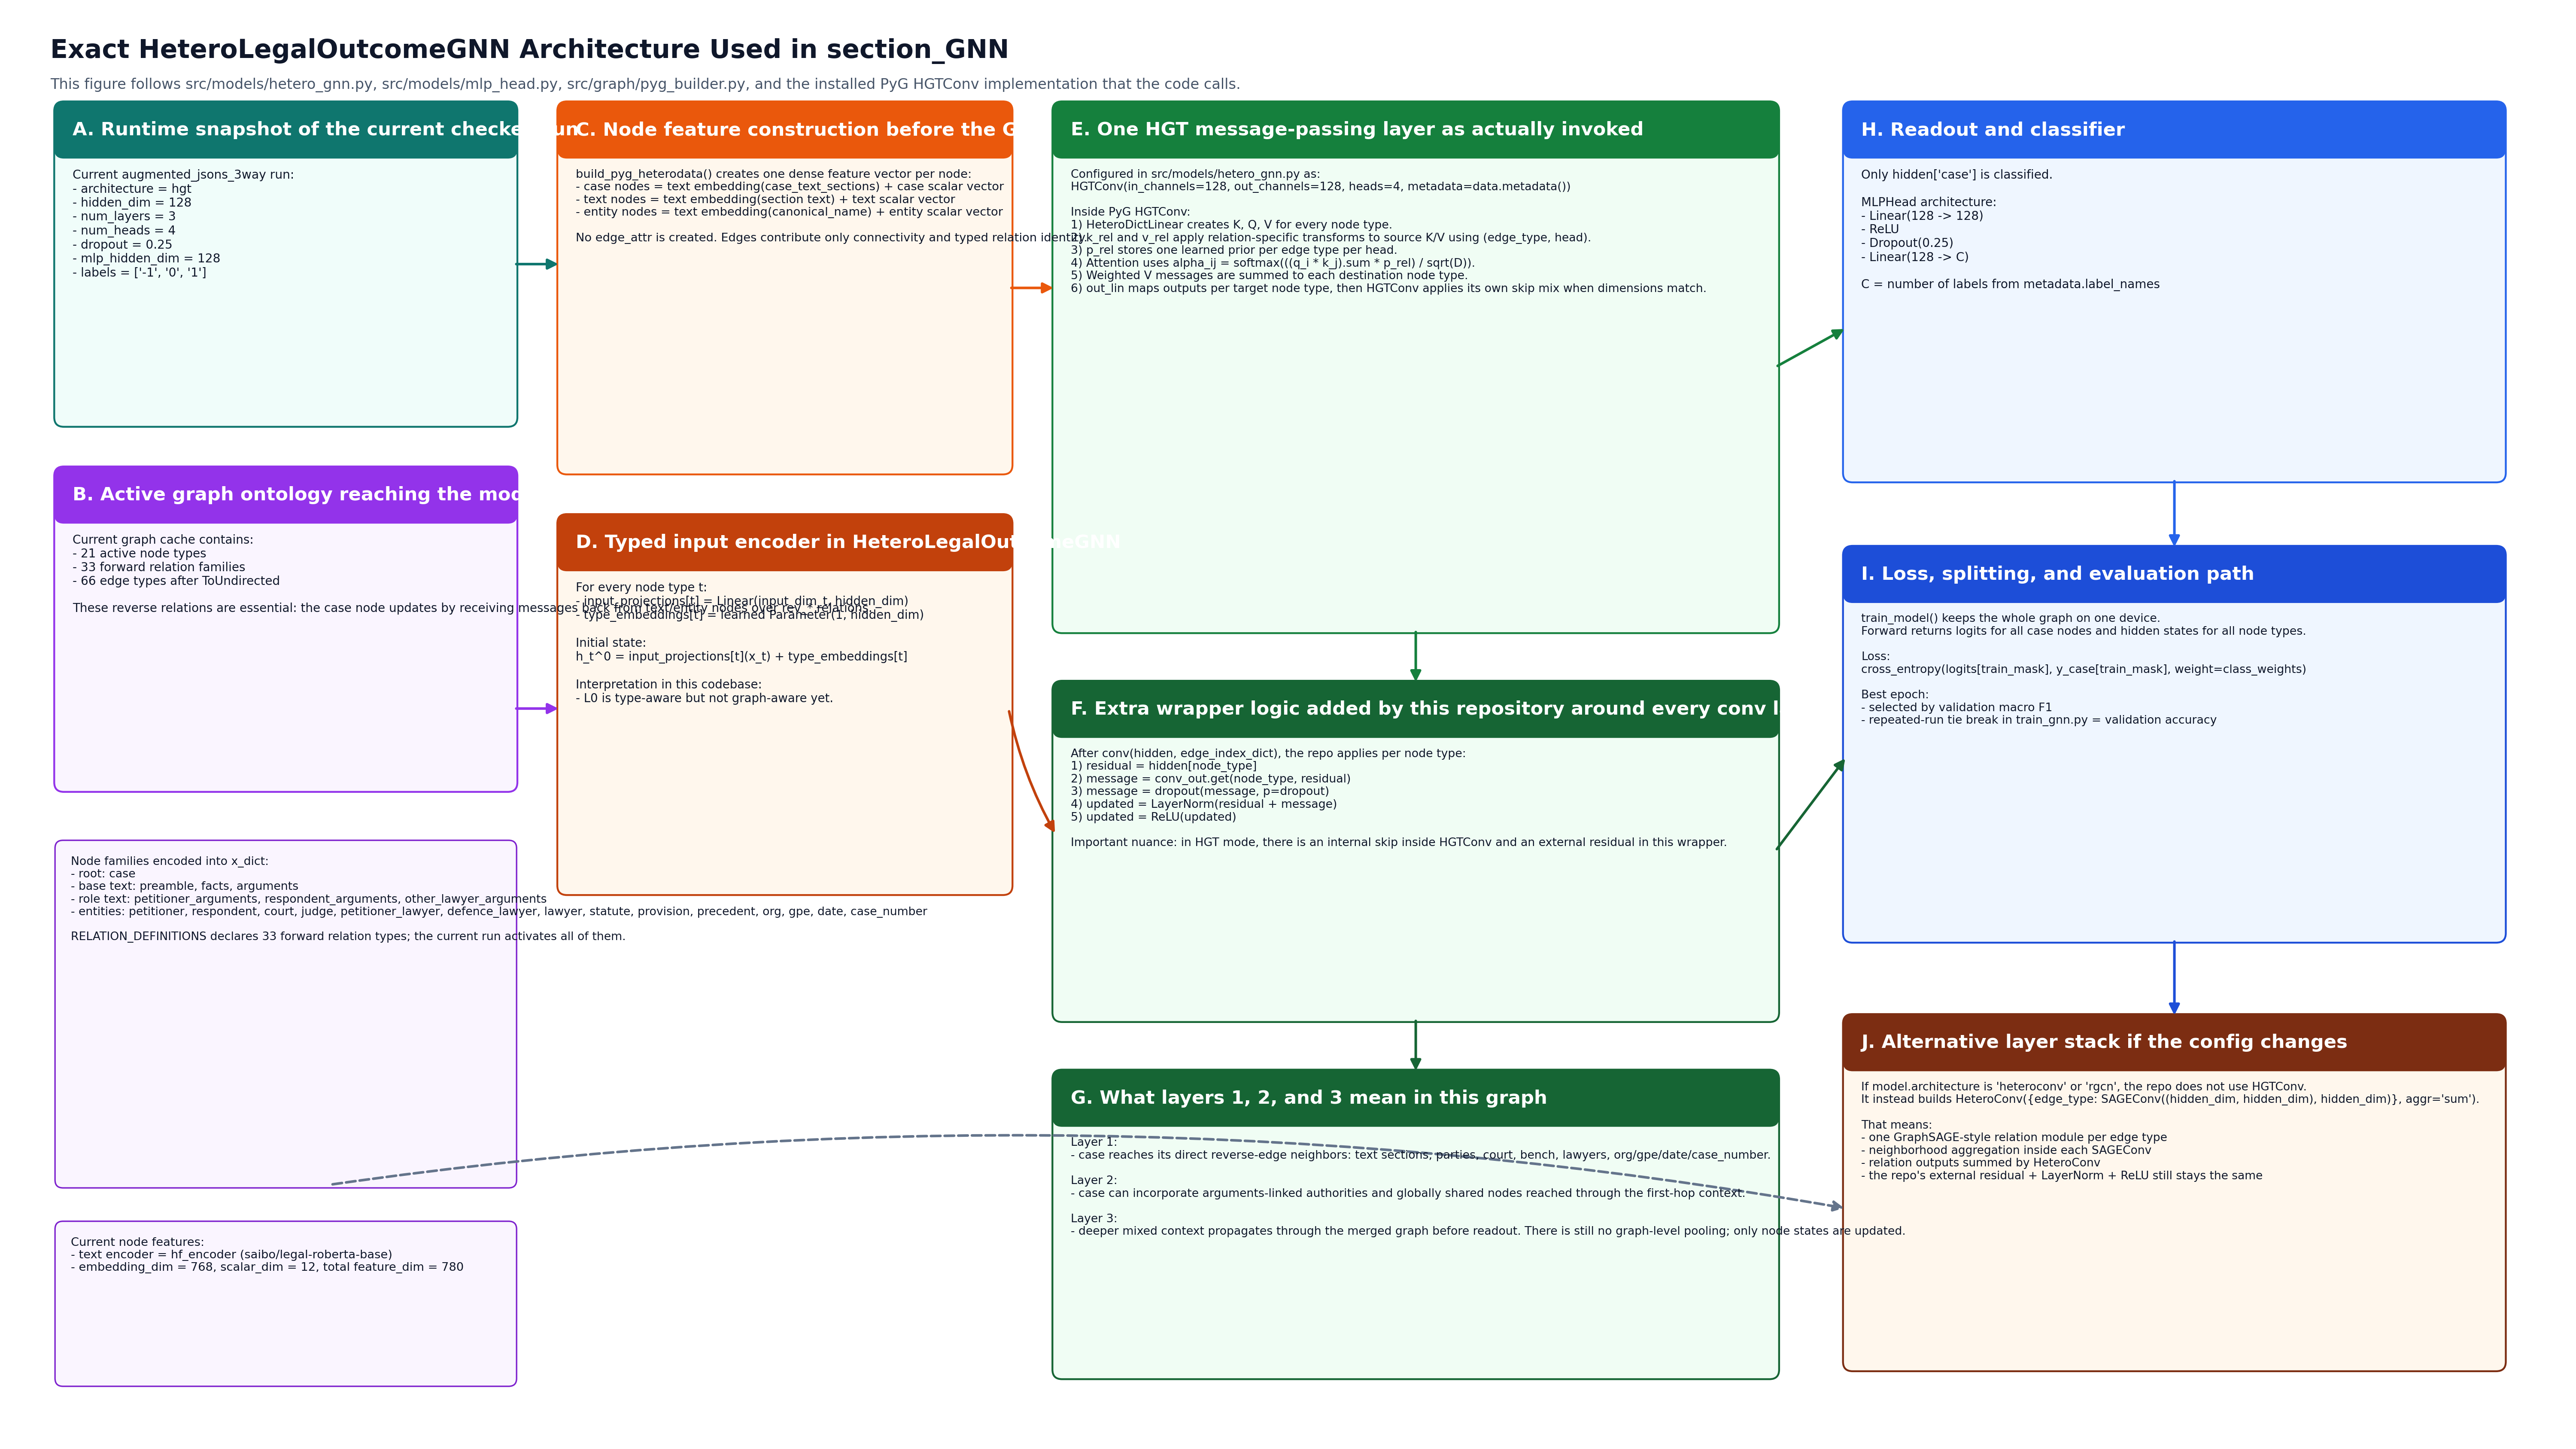
\includegraphics[width=\textwidth]{figures/section_gnn_gnn_architecture.png}
  \caption{Exact \code{HeteroLegalOutcomeGNN} architecture used by \repo{}, including feature construction, typed input projection, the invoked \code{HGTConv} mechanics, the repository's extra residual/\code{LayerNorm}/\code{ReLU} wrapper, case-only readout, and the alternate \code{HeteroConv(SAGEConv)} branch.}
  \label{fig:section-gnn-architecture}
\end{figure}

\subsection{Architecture Components}

\begin{longtable}{>{\raggedright\arraybackslash}p{0.24\textwidth}p{0.22\textwidth}p{0.44\textwidth}}
\toprule
Component & Implemented Form & Purpose \\
\midrule
\endfirsthead
\toprule
Component & Implemented Form & Purpose \\
\midrule
\endhead
\bottomrule
\endfoot
Input projection & one \code{nn.Linear(input_dim, hidden_dim)} per node type & Brings all node types to the same hidden width before message passing. \\
Type embedding & one learned \code{nn.Parameter(1, hidden_dim)} per node type & Adds a trainable type-specific offset after projection. \\
Layer normalization & one \code{LayerNorm(hidden_dim)} per node type per layer & Normalizes residual-updated activations after each message-passing layer. \\
Convolution stack & either repeated \code{HGTConv} layers or repeated \code{HeteroConv} blocks containing one \code{SAGEConv} per edge type & Performs heterogeneous message passing. \\
Classifier & \code{MLPHead(in\_dim=hidden\_dim, hidden\_dim=mlp\_hidden\_dim, out\_dim=num\_classes)} & Maps the final case-node embedding to class logits. \\
\end{longtable}

\subsection{Which Layer Types Actually Exist}
There are three categories of layers in the implemented network:

\begin{enumerate}
  \item \textbf{Input layers:} type-specific linear projections and type embeddings.
  \item \textbf{Message-passing layers:}
  \begin{itemize}
    \item \code{HGTConv} when \code{model.architecture = hgt},
    \item \code{HeteroConv} with per-relation \code{SAGEConv} when \code{model.architecture = heteroconv} or \code{rgcn}.
  \end{itemize}
  \item \textbf{Readout layers:} the two-layer MLP head.
\end{enumerate}

No other layer families are implemented. Specifically, the code does not include:

\begin{itemize}
  \item attention pooling layers,
  \item graph-level pooling layers,
  \item edge-feature encoders,
  \item jump knowledge,
  \item residual gates,
  \item batch normalization,
  \item explicit RGCN basis decomposition.
\end{itemize}

\subsection{Architecture Variants}

\begin{center}
\begin{tabular}{lp{0.62\textwidth}}
\toprule
\code{model.architecture} & Actual implementation \\
\midrule
\code{hgt} & A stack of \code{HGTConv(hidden\_dim, hidden\_dim, metadata, heads=num\_heads)}. This is the primary intended model. \\
\code{heteroconv} & A stack of \code{HeteroConv}, each containing one \code{SAGEConv((hidden\_dim, hidden\_dim), hidden\_dim)} for every edge type, aggregated by sum. \\
\code{rgcn} & Same implementation as \code{heteroconv}. It is an alias in config naming only; it is not a separate true RGCN implementation. \\
\bottomrule
\end{tabular}
\end{center}

For the \code{hgt} branch, one subtle detail matters: PyG's \code{HGTConv} itself performs a learned skip mixture when input and output dimensionalities match. In this repository, the surrounding \code{HeteroLegalOutcomeGNN} code then adds another explicit residual connection followed by \code{LayerNorm} and \code{ReLU}. In other words, the default shipped HGT stack has both an internal skip inside \code{HGTConv} and an external skip in the repository wrapper.

\subsection{Forward Pass in Detail}
The implemented \code{forward(x\_dict, edge\_index\_dict)} logic is:

\begin{enumerate}
  \item \textbf{Encode inputs.}
  For each node type:
  \[
  h_{type}^{(0)} = W_{type} x_{type} + e_{type}
  \]
  where \(W_{type}\) is the node-type-specific linear projection and \(e_{type}\) is the learned type embedding.

  \item \textbf{Repeat for each layer \(l = 1 \dots L\).}
  \begin{enumerate}
    \item cache \code{residual = hidden},
    \item compute \code{conv\_out = conv(hidden, edge\_index\_dict)},
    \item for each node type:
    \begin{enumerate}
      \item if the convolution returned an update for that node type, use it; otherwise fall back to the residual tensor for that node type,
      \item apply dropout to the message tensor,
      \item add the residual tensor,
      \item apply the node-type-specific layer norm for this layer,
      \item apply \code{ReLU}.
    \end{enumerate}
  \end{enumerate}

  \item \textbf{Read out case logits.}
  The final hidden state of \code{hidden["case"]} is passed through the MLP head:
  \[
  \text{logits} = \text{MLPHead}(h_{\text{case}}^{(L)})
  \]

  \item \textbf{Return values.}
  The model returns a tuple:
  \begin{itemize}
    \item logits for all case nodes,
    \item the full final hidden-state dictionary for all node types.
  \end{itemize}
\end{enumerate}

\subsection{Reset Logic}
\code{reset\_parameters()} resets:

\begin{itemize}
  \item every input projection,
  \item every layer norm,
  \item every convolution layer if it exposes \code{reset\_parameters()},
  \item every module inside the classifier,
  \item and initializes type embeddings from a normal distribution with mean 0 and standard deviation 0.02.
\end{itemize}

\subsection{Default Hyperparameters in Current Shipped Runs}

\begin{center}
\begin{tabular}{lrrrrr}
\toprule
Config & Hidden dim & Layers & Heads & Dropout & MLP hidden \\
\midrule
\code{gnn_case_star.yaml} & 128 & 3 & 4 & 0.25 & 128 \\
\code{gnn_case_star_food_law_final.yaml} & 128 & 3 & 4 & 0.25 & 128 \\
\code{gnn_case_star_augmented_jsons_3way.yaml} & 128 & 3 & 4 & 0.25 & 128 \\
\code{gnn_case_star_sanity.yaml} & 96 & 2 & 4 & 0.20 & 96 \\
\bottomrule
\end{tabular}
\end{center}

\section{Training, Evaluation, and Output Artifacts}

\subsection{Training Loop Behavior}
\code{train_model()} in \code{src/training/train.py} performs full-graph training:

\begin{enumerate}
  \item move the full \code{HeteroData} object to \code{cuda} if available, otherwise \code{cpu},
  \item derive each node type's input dimension from \code{data[node\_type].x.shape[1]},
  \item instantiate \code{HeteroLegalOutcomeGNN},
  \item create an \code{AdamW} optimizer,
  \item optionally compute class weights from the training labels using \code{sklearn.utils.class_weight.compute_class_weight()},
  \item for each epoch:
  \begin{enumerate}
    \item compute case logits for the entire graph,
    \item apply cross-entropy loss only on \code{logits[train\_mask]},
    \item backpropagate and step the optimizer,
    \item recompute logits in eval mode,
    \item compute train and val metrics,
    \item update the best model when validation macro F1 improves or ties the best so far,
    \item record history and possibly early-stop.
  \end{enumerate}
  \item reload the best state,
  \item compute final train/val/test metrics on that best state,
  \item build a per-case prediction table.
\end{enumerate}

\subsection{Optimization Settings}

\begin{tabularx}{\textwidth}{>{\raggedright\arraybackslash}p{0.28\textwidth}X}
\toprule
Setting & Implemented Behavior \\
\midrule
Optimizer & \code{torch.optim.AdamW} \\
Learning rate & \code{training.lr} from config \\
Weight decay & \code{training.weight_decay} from config \\
Loss & \code{F.cross_entropy} on case-node logits indexed by \code{train_mask} \\
Class weights & only when \code{training.class_weight == balanced}; otherwise no class weighting \\
Early stopping & based on patience over validation macro F1, if \code{use_early_stopping} is true \\
Device & single-device full graph, no minibatching \\
\bottomrule
\end{tabularx}

\subsection{Evaluation Metrics}
\code{compute_metrics()} returns:

\begin{itemize}
  \item \code{n_samples}
  \item \code{accuracy}
  \item \code{macro_f1}
  \item \code{micro_f1}
  \item \code{confusion_matrix}
  \item \code{classification_report}
  \item \code{per_class} precision/recall/F1/support
  \item binary only:
  \begin{itemize}
    \item \code{roc_auc}
    \item \code{pr_auc}
  \end{itemize}
  \item multiclass only:
  \begin{itemize}
    \item \code{roc_auc_ovr_macro}
  \end{itemize}
\end{itemize}

\subsection{Model Selection Rule}
The model-selection rule is explicit:

\begin{itemize}
  \item best checkpoint inside a single run: highest validation macro F1,
  \item best run across repeated runs in \code{scripts/train_gnn.py}: highest validation macro F1, with validation accuracy as the tie-breaker.
\end{itemize}

\subsection{Prediction Table Schema}
\code{predictions.csv} contains:

\begin{itemize}
  \item \code{case_id}
  \item \code{file_name}
  \item \code{raw_label}
  \item \code{split}
  \item \code{target_index}
  \item \code{target_label}
  \item \code{pred_index}
  \item \code{pred_label}
  \item \code{confidence}
\end{itemize}

In the checked 3-way run, \code{target_label} and \code{pred_label} are the strings \code{-1}, \code{0}, and \code{1}; the corresponding \code{target_index} and \code{pred_index} are \code{0}, \code{1}, and \code{2}.

\subsection{Artifacts Written Per Training Run}

\begin{tabularx}{\textwidth}{>{\raggedright\arraybackslash}p{0.29\textwidth}X}
\toprule
Artifact & Producer and Meaning \\
\midrule
\code{model.pt} & Saved state dict from the best checkpoint. It is not a full serialized model object. \\
\code{metrics.json} & Full metric dictionary including train/val/test metrics, best epoch, best validation macro F1, and epoch history. \\
\code{run_config_snapshot.yaml} & Config snapshot used for that run. \\
\code{history.csv} & Tabular copy of the epoch history inside \code{metrics.json}. \\
\code{predictions.csv} & One prediction row per retained case node. \\
\code{training_history.png} & Plot of train loss and train/val macro F1 by epoch. \\
\code{split_metrics.png} & Bar plot of accuracy, macro F1, and micro F1 for train/val/test. \\
\code{confusion_matrix_train.png} & Train confusion matrix if that split is non-empty. \\
\code{confusion_matrix_val.png} & Validation confusion matrix if that split is non-empty. \\
\code{confusion_matrix_test.png} & Test confusion matrix if that split is non-empty. \\
\code{multi_run_summary.json} & Only for repeated runs. Records all runs, best-run label, selection metric, and tie-breaker. \\
\code{best_run_config_snapshot.yaml} & Only for repeated runs. The config snapshot corresponding to the selected best run. \\
\bottomrule
\end{tabularx}

\subsection{Repeated-Run Behavior}
When \code{training.repeat_runs > 1}:

\begin{itemize}
  \item seeds are generated as \code{base_seed + run_index * seed_stride},
  \item each run writes its own directory under \code{models/<run_name>/repeats/},
  \item the best run is copied into the parent run directory.
\end{itemize}

This is how the checked binary food-law run was produced: three runs with seeds 42, 43, and 44 were trained, and the seed-44 run was selected as best.

\section{Configurations and Experiment Variants}

\subsection{Config Files Shipped in the Repository}

\begin{longtable}{>{\raggedright\arraybackslash}p{0.28\textwidth}p{0.18\textwidth}p{0.44\textwidth}}
\toprule
Config file & Main task & Distinguishing properties \\
\midrule
\endfirsthead
\toprule
Config file & Main task & Distinguishing properties \\
\midrule
\endhead
\bottomrule
\endfoot
\code{configs/gnn_case_star.yaml} & base binary config & Older base config with absolute paths into a sibling \code{GNN/} directory tree, binary labels, MiniLM text encoder, HGT backbone, ablation variants, and no role-specific argument nodes in the graph. \\
\code{configs/gnn_case_star_food_law_final.yaml} & binary food-law run & Uses \code{section_GNN} paths, enables role-specific argument nodes in the graph, MiniLM sentence-transformer embeddings, repeated runs (\code{repeat_runs: 3}), and no early stopping. \\
\code{configs/gnn_case_star_augmented_jsons_3way.yaml} & 3-way classification & Uses \code{section_GNN} paths, role-specific argument nodes, Hugging Face encoder backend \code{saibo/legal-roberta-base}, class labels \code{-1}/\code{0}/\code{1}, and one training run. \\
\code{configs/gnn_case_star_sanity.yaml} & fast sanity check & Uses hashing embeddings, smaller hidden size, fewer layers, fewer epochs, and simpler paths into an older \code{GNN/} tree. \\
\end{longtable}

\subsection{Ablation Variants}
The base and food-law configs define ablation variants under \code{ablation.variants}. The variants currently shipped are:

\begin{itemize}
  \item \code{text_only}
  \item \code{star_only}
  \item \code{full_star_global}
  \item \code{without_judge}
  \item \code{without_statute_provision}
  \item \code{without_preamble}
  \item \code{facts_only}
  \item \code{arguments_only}
\end{itemize}

These are implemented as config overrides merged onto the base config by \code{deep_merge_dict()} inside \code{run_ablation.py}.

\subsection{Features Config Differences Across Variants}

\begin{center}
\begin{tabular}{lccc}
\toprule
Config & Text backend & Embedding dim in current artifacts & Scalar dim \\
\midrule
\code{food_law_final} & \code{sentence_transformers/all-MiniLM-L6-v2} & 384 & 12 \\
\code{augmented_jsons_3way} & \code{saibo/legal-roberta-base} via \code{hf_encoder} & 768 & 12 \\
\code{sanity} & \code{hashing} & 384 & 12 \\
\bottomrule
\end{tabular}
\end{center}

\section{Visualization Subsystem}

\subsection{Static Figure Generation}
The repository contains a separate static-visualization subsystem that is not used during model training:

\begin{itemize}
  \item \code{scripts/visualize_graph.py}
  \item \code{scripts/generate_final_visualisations.py}
  \item \code{src/visualization/graph_visualizer.py}
  \item \code{src/visualization/final_visualizer.py}
\end{itemize}

These modules generate explanatory PNG figures such as:

\begin{itemize}
  \item graph schema diagrams,
  \item local case star views,
  \item receptive-field visualizations,
  \item message-passing cartoons,
  \item ``what is stored in vertices'' and ``what is stored on edges'' explanations,
  \item layer-1 and layer-2 update illustrations,
  \item README-style Markdown summaries beside the figures.
\end{itemize}

\subsection{Browser Visualizer}
The \code{visualiser/} directory contains a static browser application:

\begin{itemize}
  \item \code{visualiser/index.html}: main D3 graph view,
  \item \code{visualiser/stats/index.html}: stats dashboard,
  \item \code{visualiser/layers/index.html}: graph/model layer explainer,
  \item \code{visualiser/data/cases_catalog.js}: sampled fallback catalog,
  \item \code{visualiser/data/training_graph/}: exact exported training graph details for browser loading.
\end{itemize}

The new exporter \code{scripts/export_training_graph_visualiser.py} rebuilds exact local case-star graphs for browser display by:

\begin{enumerate}
  \item loading the effective config, preferring \code{graph_config_snapshot.yaml} if present,
  \item loading filtered cleaned cases,
  \item restricting to case ids present in \code{split_assignments.json},
  \item calling the same \code{build_case_star_graph()} logic used by the training pipeline,
  \item writing an index file and one JSON detail file per case.
\end{enumerate}

This is a documentation/inspection tool. It does not affect training.

\section{Current Artifact Snapshot}

\subsection{Binary Food-Law Run}
From \code{data/food_law_final/graph_cache/graph_metadata.json} and
\code{outputs/food_law_final/models/food_law_final_section/metrics.json}:

\begin{itemize}
  \item retained cases: 1466
  \item dropped procedural cases: 639
  \item feature dimension: 396 = 384 embedding + 12 scalar
  \item node types present: 21
  \item relation types present after \code{ToUndirected}: 66
  \item split sizes: train 1026, val 220, test 220
  \item selected best repeated run: \code{run_03_seed_44}
\end{itemize}

\begin{center}
\begin{tabular}{lrrr}
\toprule
Split & Accuracy & Macro F1 & Samples \\
\midrule
Train & 0.9951 & 0.9944 & 1026 \\
Val & 0.8591 & 0.8300 & 220 \\
Test & 0.7636 & 0.7108 & 220 \\
\bottomrule
\end{tabular}
\end{center}

\subsection{3-Way Augmented-JSONs Run}
From \code{data/augmented_jsons_3way/graph_cache/graph_metadata.json} and
\code{outputs/augmented_jsons_3way/models/augmented_jsons_3way/metrics.json}:

\begin{itemize}
  \item retained cases: 2105
  \item dropped cases: 0
  \item label distribution after filtering:
  \begin{itemize}
    \item \code{appellant_lost}: 459
    \item \code{postponed_or_procedural}: 639
    \item \code{appellant_won}: 1007
  \end{itemize}
  \item feature dimension: 780 = 768 embedding + 12 scalar
  \item node types present: 21
  \item relation types present after \code{ToUndirected}: 66
  \item split sizes: train 1473, val 316, test 316
\end{itemize}

\begin{center}
\begin{tabular}{lrrr}
\toprule
Split & Accuracy & Macro F1 & Samples \\
\midrule
Train & 0.9722 & 0.9715 & 1473 \\
Val & 0.7215 & 0.6961 & 316 \\
Test & 0.7215 & 0.6937 & 316 \\
\bottomrule
\end{tabular}
\end{center}

\subsection{Observed Graph Scale in Current Artifacts}
The current graph caches are large enough that scale matters for implementation and performance:

\begin{itemize}
  \item in the binary food-law cache, \code{petitioner} nodes number 123{,}341 and \code{respondent} nodes number 109{,}561 for only 1466 retained cases;
  \item in the 3-way cache, \code{petitioner} nodes number 126{,}021 and \code{respondent} nodes number 114{,}275 for 2105 retained cases;
  \item in both caches, place and organization mentions create very dense case-to-context edges.
\end{itemize}

This strongly suggests that party normalization remains noisy and that many party nodes are effectively near-unique.

\section{Limitations, Ambiguities, and Extension Points}

\subsection{Code-Grounded Limitations}

\begin{enumerate}
  \item \textbf{Leakage prevention is phrase-driven.} The leakage detector is a list of literal regex phrases. It can miss unseen wording of outcome-bearing text.

  \item \textbf{Lawyer-side assignment is heuristic.} \code{_infer_lawyer_side()} uses a fixed local text window and signal phrases. Misassignment is possible when formatting is unusual.

  \item \textbf{Party normalization appears weak in practice.} Current graph caches contain extremely large numbers of unique petitioner and respondent nodes relative to case count.

  \item \textbf{No edge features exist.} Relation type and connectivity are the only edge information used by the model.

  \item \textbf{Training is fully transductive.} Shared nodes connect train, val, and test cases inside one graph. This is by design, but it matters when interpreting generalization.

  \item \textbf{No minibatching or neighbor sampling.} The entire graph is loaded onto one device each epoch.

  \item \textbf{The embedding cache key is not content-safe.} It uses ids and text lengths, not the full text content.

  \item \textbf{\code{sentence_transformers} backend ignores some config fields.} In the current implementation, the sentence-transformer backend does not use the configured \code{pooling} value and does not explicitly pass \code{max_length}.

  \item \textbf{Grouped splits are not stratified.} \code{year} and \code{court} modes use \code{GroupShuffleSplit}, which preserves groups but not class balance.
\end{enumerate}

\subsection{Config and Schema Drift}

\begin{enumerate}
  \item \textbf{\code{include_reverse_edges} exists in YAML but is not read by the runtime code.} Reverse edges are actually controlled by \code{graph.use_to_undirected}.

  \item \textbf{\code{allowed_summary_fields} exists in YAML but is not used directly in \code{extract_prejudgment_text()}.} The implementation reads a fixed \code{SECTION_NAME_MAP} of \code{PREAMBLE}, \code{facts}, and \code{arguments}.

  \item \textbf{\code{RELATION_DEFINITIONS} is declarative but not authoritative at runtime.} The actual edge creation logic is hard-coded inside \code{case_star_builder.py}. Changing only \code{RELATION_DEFINITIONS} does not change the graph.

  \item \textbf{\code{rgcn} is a naming alias, not a real separate implementation.} It uses the same \code{HeteroConv + SAGEConv} path as \code{heteroconv}.
\end{enumerate}

\subsection{Extending the Graph Schema}
To add a new entity/node family cleanly, the implementation currently requires coordinated edits in multiple places:

\begin{enumerate}
  \item map the upstream label in \code{src/preprocessing/extract.py},
  \item normalize the new entity type in \code{src/preprocessing/normalize.py} if needed,
  \item add the node type constant in \code{src/graph/schema.py},
  \item decide whether it is shareable and add it to relevant YAML configs,
  \item create node and edge construction logic in \code{src/graph/case_star_builder.py},
  \item extend scalar-feature logic in \code{src/graph/pyg_builder.py} if the new node family needs extra structured features,
  \item update browser/static visualization code if the new type should be inspectable there.
\end{enumerate}

\subsection{High-Value Extension Points}

\begin{itemize}
  \item replace phrase-based leakage masking with stronger semantic leakage detection,
  \item improve party normalization and canonicalization,
  \item add explicit edge features or edge weights,
  \item introduce case-local or temporal split regimes that avoid a single transductive global graph,
  \item add a real RGCN or other hetero backbones rather than aliasing \code{rgcn} to \code{HeteroConv},
  \item make the embedding cache key content-sensitive,
  \item add batching or neighbor-sampling support for larger graphs,
  \item centralize the graph schema so that \code{RELATION_DEFINITIONS} becomes executable rather than purely descriptive.
\end{itemize}

\section{Summary}
\repo{} is a fairly clean end-to-end heterogeneous legal GNN pipeline with three strong design choices:

\begin{enumerate}
  \item it explicitly treats pre-judgment leakage as a first-class preprocessing concern,
  \item it separates local case-star structure from global cross-case sharing,
  \item it keeps training simple and inspectable by using a single full-graph supervised objective on case nodes.
\end{enumerate}

Its most important implementation realities are equally clear:

\begin{itemize}
  \item the graph ontology and forward relations are richer than the initial documentation suggested,
  \item the shipped experiments already include role-specific argument nodes and typed lawyer-to-argument bridges,
  \item the current system is transductive, full-graph, and mostly relation-driven rather than edge-feature-driven,
  \item several configuration keys are descriptive only and do not yet fully govern runtime behavior.
\end{itemize}

That is the repository as implemented today.

\end{document}
